%************************************************
\chapter[Modèle et simulation]{Modèle morphologique et simulation de scènes sonores environnementales}\label{ch:psycho_model} 
%************************************************

\section{Introduction}

Nous appuyant sur les connaissances relatives au fonctionnement du système auditif présentées au chapitre précédent (\cf~Chapitre~\ref{ch:psycho_ea}), nous développons, en phase préliminaire à nos travaux, un modèle morphologique de scènes sonores environnementales. Il ne s'agit pas ici de proposer un modèle analytique de scènes sonores au sens physique ou psychophysique, mais plutôt de satisfaire à un intérêt pratique, \ie~proposer un modèle permettant de facilement simuler des scènes sonores dont nous contrôlons les caractéristiques structurelles. Ces caractéristiques sont supposées être des facteurs importants entrant en compte dans l'analyse des scènes, qu'il s'agisse d'analyse sensorielle, ou d'analyse automatique.


Ce chapitre comprend trois sections. La première explicite les considérations perceptives sur lesquelles s'ancre le modèle. La seconde présente une formalisation du modèle morphologique. La troisième motive l'utilisation du modèle dans le cadre des deux cas d'étude choisis: la perception de l'agrément dans un milieu urbain, et l'évaluation des algorithmes de détection d'événements sonores.

\section{Fondement perceptif du modèle morphologique}
\label{sec:ch4_model}

\subsection{L'unité: la source sonore}

Les études portant sur l'ASA, et plus spécifiquement sur les processus de ségrégation, montrent, d'une part, que l'homme fait sens de son environnement en isolant les informations relatives aux différentes sources qui le composent, d'autre part, que ce groupement intervient très tôt dans la chaîne de traitement, et se base sur des règles génériques innées (\cf~Section~\ref{sec:ch3_ASA}).

Dans le même temps, l'approche de l'ASA par les neurosciences montre que le système auditif tend à générer des images mentales (« objets auditifs\,'') des sources ainsi isolées, et que c'est à partir de ces images qu'il adapte son traitement de l'information montante (\cf~Section~\ref{sec:ch3_asaNeuro}).

Enfin, la recherche sur les paysages sonores, adoptant l’approche catégorielle, met en évidence que les processus de catégorisation s'appuient également sur la composition sémantique des scènes, \ie~les sources sonores identifiées (\cf~Section~\ref{sec:ch3_catsoundscape}). 

Pour modéliser un environnement sonore, il semble pertinent de considérer comme élément de base la source sonore. Comme vu précédemment (\cf~Section~\ref{sec:ch3_categoEtAbstract}), la notion de source sonore est variable, un même objet pouvant être reconnu suivant plusieurs degrés d'abstraction.

\subsection{L'objet: la séquence sonore}

Les études portant sur l'ASA (psychophysiques et neurosciences), montrent que des événements émis par une même source ont tendance à être groupés dans un même flux, et traités comme une seule entité, par le système auditif (\cf~Section~\ref{sec:ch3_asaFlux}).

Par ailleurs, la nature catégorielle des représentations mentales suggère encore cette tendance \emph{a priori} naturelle de l'homme à considérer comme équivalents des objets partageant un certain nombre de propriétés en commun (\cf~Section~\ref{sec:ch3_representationMentale}).

De fait, il n'apparaît pas nécessaire, pour le modèle, de gérer séparément deux éléments sonores proches et relevant d'une même source. Ces éléments sont regroupés dans une séquence sonore. Cette séquence forme l'objet de base du modèle, celui dont nous contrôlons les caractéristiques. 

\subsection{Une typologie source-action}
\label{sec:ch4_sourceAction}

La constitution de banques de sons peuplant l'environnement urbain est incontournable. Avant d'acquérir ces sources, \ie~de les enregistrer, il est nécessaire de les identifier. Une démarche naïve consisterait alors à établir la liste exhaustive de toutes les classes de sources sonores composant l'environnement. Une telle approche soulèverait deux problèmes:

\begin{itemize}
\item une source sonore peut se décrire en fonction de plusieurs niveaux d'abstraction. Identifier et nommer sont des actions déterminées par notre représentation mentale du monde (\cf~Section~\ref{sec:ch3_representationMentale}). Cette représentation s'organise, entre autre, suivant l'axe vertical des niveaux d'abstraction sur lequel s'appuie notre travail de catégorisation. Ainsi, si deux individus entendent un même son de voiture, il est possible que le premier le nomme « voiture~» et le deuxième « moteur~». Le dénombrement de l'ensemble des sources pouvant être utilisées par le modèle doit prendre en compte ce fait. Ces sources doivent être regroupées en classes hiérarchisées, afin de bâtir une structure taxonomique;
\item il n'existe pas de taxonomie standardisée des sources sonores. Pourtant, c'est une tradition des sciences modernes de classer et nommer les éléments avant de les étudier. Dans les domaines de la faune ou de la flore, une observation longue et minutieuse des sujets d'étude a permis d'élaborer un système de classification (taxonomie), et ainsi d'organiser et trier les objets en fonction de leurs propriétés partagées. Elle a permis encore d'élaborer une terminologie précise des classes d'objets. Grâce à quoi, la Biologie est devenue une science, laquelle science devait donner naissance à la théorie de l'évolution \citep{lecointre2006tree}. Dans le domaine du son, en revanche, point de système de classification \citep{dubois2000categories,niessen2010categories}. Nous trouvons à cela deux explications:

\begin{itemize}
\item \emph{champ lexical limité}: l'identification et la description d'un son sont des processus subjectifs étroitement liés au langage (\cf~Section~\ref{sec:ch3_catLang}). Deux sujets appartenant à deux groupes sociaux différents n'utiliseront pas les mêmes mots pour décrire un même objet. Pour établir un système de classification, il faut prendre une décision quant à la définition des termes utilisés. Or, contrairement au domaine de la vision, où une terminologie de base pour décrire les objets (couleur, forme etc.) est globalement partagée, le champ lexical applicable aux phénomènes acoustiques est, d'une part, limité (durée, fréquence...) \citep{dubois2000categories}, d'autre part, emprunté, dans une large mesure, à d'autres domaines perceptifs. On parle ainsi de brillance, ou de rugosité des sons. La diversité des termes descriptifs, et l'absence de consensus sur ce qu'ils désignent, rend difficile l'élaboration d'une classification standardisée;
\item \emph{influence du contexte}: L'identification et la description d'un son sont dépendantes du contexte (\cf~Section~\ref{sec:ch3_categoEtContexte}), \ie~de la nature des sources co-occurrentes dans la scène \citep{ballas1987interpreting,niessen2008disambiguating,gygi2011incongruency}.
\end{itemize}
\end{itemize}

Il apparaît clairement que les classes de sons peuplant notre environnement doivent être organisées autour d'une taxonomie: un système de classes hiérarchisé. Cependant il y a un choix à faire quant à la manière de regrouper les sons à l'intérieur de cette taxonomie.

Comme vu à la section~\ref{sec:ch3_catSourceSoundScape}, plusieurs études ont montré que la catégorisation des sources sonores s'opère suivant des attributs sémantiques. Parmi ceux-ci, deux reviennent souvent:

\begin{itemize}
\item la source (agent, objet, fonction), \ie~l'objet émettant le son;
\item l'action, \ie~le mouvement physique à l'origine du son.
\end{itemize} 

Ces deux attributs fonctionnent de pair. S'inspirant de l'organisation catégorielle verticale à trois niveaux de Rosch (\cf~Section~\ref{sec:ch3_categoEtAbstract}), Guyot et al. \citep{guyot1997} proposent un système de catégorisation où les auditeurs identifient des groupements de sources abstraites au niveau superordonné (« Bruit généré par une excitation mécanique~»), des actions au niveau de base (« gratter~»,« frotter~») et des sources concrètes au niveau subordonné (« vaisselle~»,« stylo~»). Reprenant à son tour ce système, \citep{houix_lexical_2012} montre que les sons sont catégorisés, en premier lieu, à partir du type de sources concrètes, et ensuite, seulement, à partir d'actions.

L'association source-action semble être une base sensée sur laquelle bâtir une taxonomie où les classes haut-niveau sont des classes abstraites de sources sonores (« véhicule~»), les classes intermédiaires, des classes de sources sonores (« voiture~»), et les classes basses, des actions sonores (« passage~»). Pour les classes de bas niveau, la perméabilité intra-classe est minimale.

Cette association source-action n'est cependant pas suffisante. Le choix des labels utilisés doit faire l'objet d'une sélection particulière. Ces labels doivent être génériques, compréhensibles, et décrire de manière non ambiguë les objets de la classe considérée. Afin de les déterminer, il est possible de se référer aux travaux de Gaver \citep{gaver1993world}, qui propose une taxonomie phénoménologique des sons, à ceux de Niessen~\al \citep{niessen2010categories} qui, sur la base d'une étude bibliographique de près de 35 publications, établit la liste des catégories sonores les plus utilisées, également à ceux de Salamon~\al \citep{Salamon14}, qui, partant des travaux de \citep{brown2011towards}, et reprenant l'association source-action, élaborent une taxonomie de sons urbains.

\subsection{Événements et textures}
\label{sec:ch4_eventTextureAmorphe}

Nous avons montré que l'utilisation de la nomenclature basée sur l’association source-action nous permet de dénombrer et de trier l'ensemble des sons présents dans l'environnement.

Afin de permettre le développement d'un outil de création de scènes sonores simulées à partir d'enregistrements de sons réels, il est nécessaire de constituer un corpus d'enregistrements, corpus structuré suivant la taxonomie définie. 

Le problème est alors, sur la base de cette taxonomie, d'enregistrer, pour chacune des classes, un nombre de sons suffisant. Considérant des environnements denses comme la ville ou la forêt, cette approche pose une question pratique de faisabilité.

Afin de contourner le problème, on peut s’appuyer sur des considérations perceptives pour définir, dans un contexte expérimental donné, quels sons requièrent d'être enregistrés séparément, quels autres peuvent l'être simultanément.

En effet, tous les sons n'ont pas le même intérêt. Une voix humaine peut facilement être isolée du reste des sons concurrents \citep{carlyon2004brain}. Inversement, un fond sonore de trafic urbain est moins informatif que d'autres sons ponctuels et proches~\citep{southworth1969sonic}.
Maffiolo montre à ce sujet (\cf~Section~\ref{sec:ch3_catsoundscape}) l'existence de deux processus cognitifs distincts dont l'activation dépend de la nature des environnements: l'analyse holistique, s'agissant de scènes amorphes, \ie~sans événements apparents, et l'analyse descriptive (sur la base d'une information sémantique extraite à partir des événements connus), s'agissant de scènes événementielles, \ie~comprenant des événements identifiables.

Par ailleurs, le cerveau a tendance à résumer l'information extraite, lorsqu'il détecte qu'une séquence n'est composée que d'un mélange de sons similaires, et que ces sons n'enrichissent pas l'information. Cette particularité a déjà été évoquée (\cf~Section~\ref{sec:ch3_eventTexture}). 

Ces éléments nous amènent à penser que les processus de ségrégation dépendent de la nature structurelle de l'environnement. Lorsque des événements émergent d'un environnement sonore, le cerveau traite l'information des différentes sources de manière séparée. Plusieurs flux auditifs sont ainsi générés \ie~un pour chaque séquence d'événements émis par la même source. Inversement, quand le cerveau ne parvient pas à isoler d'événement, la scène est traitée globalement, tous ces constituants étant agglomérés dans un même flux.

Ainsi, quatre types de sons semblent pouvoir être isolés:

\begin{itemize}
\item {événement sonore}: un son isolé, ponctuel, dont les caractéristiques physiques varient au cours du temps;
\item {texture sonore}: un son, isolé, long, dont les caractéristiques physiques restent stables au cours du temps, et analysé à partir de statistiques extraites d'une représentation temps-fréquence;
\item \emph{scène événementielle}: une séquence contenant une information sémantique élevée;
\item \emph{scène amorphe}: une séquence contenant une information sémantique faible.
\end{itemize}

Une scène événementielle est une séquence composée soit uniquement d'événements, soit d'événements et de textures, les événements porteurs d'une information plus riche primant quant au choix du processus de traitement à mettre en œuvre.
 
Les textures et les scènes amorphes, elles, sont traitées de manière holistique, à partir de propriétés acoustiques globales pour les scènes amorphes \citep{dubois2006cognitive,maffiolo_caracterisation_1999}, et sur la base d'une information résumée statistiquement pour les textures \citep{mcdermott2013summary}. Toutes deux portent une information limitée \citep{saint1995classification,nelken2013ear}. Cependant, les séquences amorphes sont spontanément décrites par les sujets comme des «~fonds sonores~» \citep{maffiolo_caracterisation_1999,guastavino2006ideal}, induisant qu'elles n'existent que grâce à un processus de construction de flux auditifs, alors que les textures sont des objets définis seulement sur la base de leur nature physique. Il est cependant possible d'assimiler une scène amorphe à une texture, ses caractéristiques physiques demeurant stables au cours du temps. De fait, nombre de scènes amorphes («~brouhaha de rue~», «~brouhaha de trafic~») sont citées comme textures. Cependant, l'inverse, considérer une texture comme une scène amorphe, n'est pas forcément vrai.
Un exemple de texture souvent cité est le son du «~galop~», son qui peut très bien apparaître au premier plan de la scène.

Afin de limiter le nombre d'enregistrements nécessaire, il est donc possible d'enregistrer directement des mixtures de sons, à la condition qu'elles puissent être considérées comme des textures, la définition de cette dernière notion englobant les scènes amorphes. 

\section{Description du modèle morphologique}
\label{sec:ch4_modelDes}

\subsection{Classe et collection de samples}
\label{sec:ch4_collecSons}

La scène sonore est vue comme une somme de sources sonores, ou, si l'on admet la distinction opérée entre événements et textures sonores, «~un squelette d'événements sur un lit de textures~» \citep{nelken2013ear}. 

D'un point de vue pratique, ces éléments sonores sont enregistrés. Ils sont nommés samples.
 
\begin{mydef}
Un sample est un enregistrement d'un son isolé, qu'il s'agisse d'un événement ou d'une texture.
\end{mydef}

Les samples, regroupés en classes de sons hiérarchisées, sont organisés selon la taxonomie préétablie. Un exemple est donné figure~\ref{fig:orgDb}. Les niveaux hiérarchiques de la taxonomie sont appelés niveaux d'abstraction. Les classes ayant un niveau d'abstraction élevé constituent un regroupement conceptuel de samples ayant potentiellement des caractéristiques variées (\eg~{Humain}). Plus le niveau de la classe est bas, plus le groupement est précis, englobant des samples similaires (\eg~\emph{voix-adulte-cri}). 

\begin{mydef}
Une classe est une collection de samples jugés perceptivement équivalents. Si le niveau d'abstraction d'une classe est tel que cette dernière possède des sous-classes, alors sa collection de samples est la somme des collections respectives de chacune des sous-classes.
\end{mydef}

Les classes de niveau d'abstraction élevé sont nommées uniquement à l'aide de termes abstraits désignant, de manière globale, les samples qu'elles regroupent (\eg~\emph{transport}). Les classes de niveau moindre utilisent la nomenclature source-action (\eg~\emph{passage de voiture}). Les classes des niveaux les plus bas correspondent à des collections de samples, par définition, équivalents les uns aux autres.

\subsection{Séquences de samples}
\label{sec:ch4_seqSample}

Chaque classe de sons faisant partie de la scène est liée à une piste. Cette piste est une séquence temporelle où sont positionnés les différents samples. Elle est le correspondant simulé du flux auditif.

\begin{mydef}
Une piste est une séquence temporelle composée de samples appartenant à une même classe de sons.
\end{mydef}

La construction de la taxonomie (nombre de classes, nombre de niveaux d'abstraction), dépend, évidemment, de la tâche considérée. 

L'ensemble des pistes, ainsi que leurs paramètres, forment ce que nous appelons un scénario sonore.

\begin{mydef}
Le scénario sonore désigne l'ensemble des propriétés des pistes composant une scène, à savoir, les classes de sons liées aux pistes, et leurs paramètres structurels (niveau, espacement, début et fin, \cf~Section~\ref{sec:ch4_modelParam}).
\end{mydef}

\begin{figure}[t]
        \myfloatalign
        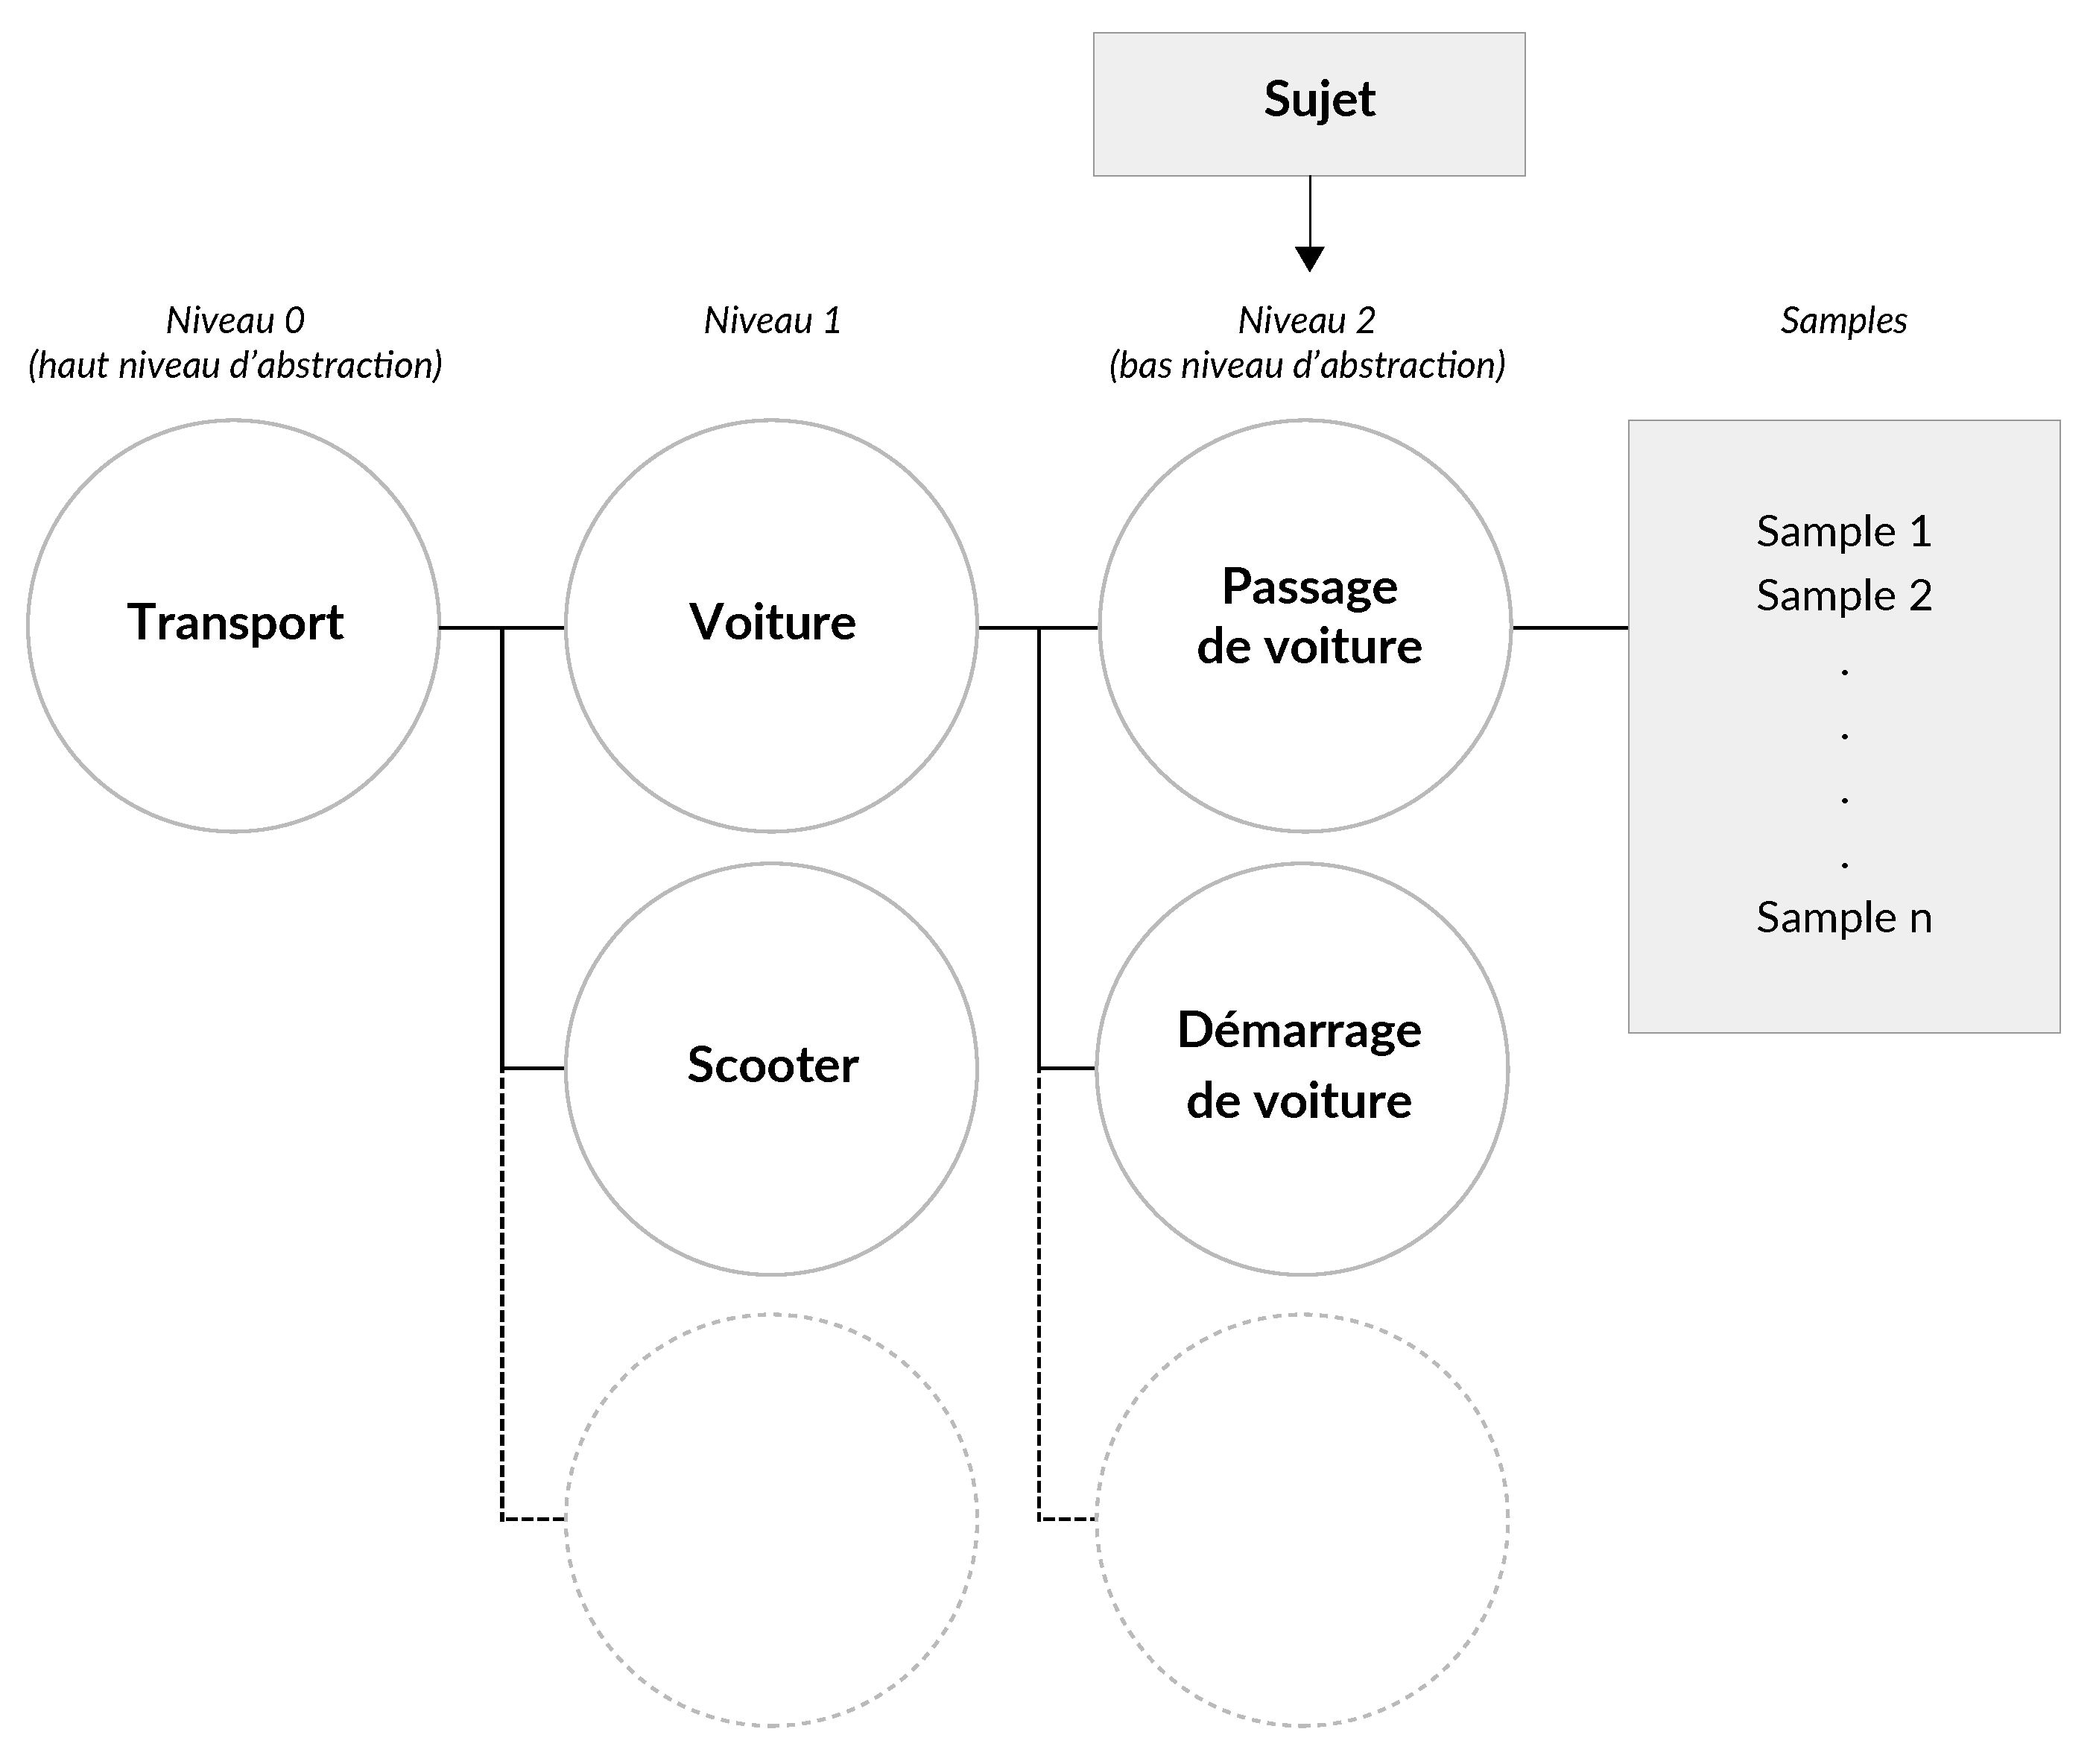
\includegraphics[width=.8\linewidth]{gfx/ch_4/3}
       \caption{Organisation hiérarchique de la banque de sons isolés utilisée pour la simulation.}\label{fig:orgDb}
\end{figure}

\subsection{Paramètres}
\label{sec:ch4_modelParam}

En suivant la terminologie ci-devant introduite, une scène sonore est vue comme une somme de pistes. Chaque piste est une séquence temporelle, dont la structure dépend d'une série de paramètres (\cf~Figure~\ref{fig:modelSequence}). Une description exhaustive de la scène supposerait de connaître au moins les positions et les niveaux exacts de chaque occurrence de chaque sample. Ces informations seraient trop nombreuses pour être correctement maîtrisées et interprétées. Nous proposons donc de réaliser une approximation en posant l'hypothèse d'une distribution normale des valeurs. Le modèle ne propose pas d’interagir avec un sample en particulier, mais toujours avec une séquence de samples.

Nous isolons trois attributs globaux permettant de contrôler une piste:

\begin{itemize}
\item \emph{niveau}: la moyenne/variance des niveaux des samples;
\item \emph{espacement}: la moyenne/variance des espacements inter-\emph{onsets} entre les samples;
\item \emph{durée}: le début et la fin de la piste.
\end{itemize}

Le modèle fait une distinction explicite entre la gestion des pistes d'événements, et la gestion des pistes de textures. En effet, la notion de texture ne peut se comprendre que pour un son continu. Une piste de texture est donc composée de samples concaténés les uns aux autres, sans espacement (\cf~figure~\ref{fig:modelSequence}). Pour qu'une piste de texture soit «~plausible~», \ie~qu'on ne détecte pas de discontinuité flagrante, elle doit être une séquence composée de samples provenant de la même source, et obtenus avec un matériel (et des réglages) identique(s).

Le scénario sonore est défini à partir de paramètres stochastiques. Il existe une infinité de réalisations pour un scénario donné. Nous nommons partition, une réalisation particulière d'un scénario.

\begin{mydef}
La partition désigne l'ensemble des propriétés des samples composant une réalisation particulière d'un scénario sonore donné (classe, niveau, \emph{onsets} et \emph{offsets} de chacun des samples).
\end{mydef}

\begin{figure}[t]
        \graphicspath{{gfx/ch_4/}}
        \myfloatalign
        \def\svgwidth{\linewidth}
        \input{gfx/ch_4/controlParameters2.pdf_tex}
       \caption{Représentation schématisée des pistes du modèle de scènes sonores.}\label{fig:modelSequence}
\end{figure}


\subsection{Formalisation du modèle}
 \label{sec:ch4_modelForm}
 
La formalisation présentée ici vaut uniquement pour les classes d'événements sonores. Nous décrivons par la suite les diverses contraintes qui s'appliquent pour une classe de textures.
 
En considérant $s$, une scène composée de $z$ classes de sons, le modèle de $s$ se définit comme suit:
 
\begin{equation}
s(n)=\sum_{i=1}^{z}p_i(n)
\end{equation}

avec $n$ un indice temporel discret, et $p_i$ la piste correspondant à la classe $c_i$. La classe $c_i$ est composée de $\vert c_i\vert$ samples $c_{i,m}$, $1<m<\vert c_i\vert$. 

Soit $\mathcal{U}(x,y)$, une distribution uniforme d'entiers allant de $x$ à $y$, avec $x<y$. On définit $E_j^i$ ($j=\lbrace 1,2,\ldots,k_i\rbrace$) une suite de variables aléatoires indépendantes et identiquement distribuées (iid) suivant la loi $\mathcal{U}(1,\vert c_i \vert)$.

\begin{equation}
E_j^i \textrm{ iid : } \mathcal{U}(1,\vert c_i \vert) \quad \forall j 
\end{equation}

Une piste $p_i$ est vue comme une séquence de $k_i$ samples d'événements. On définit $e_j^i(n)$, un événement choisi aléatoirement parmi les $\vert c_i\vert$ samples de la classe $c_i$ :

\begin{equation}
e_j^i=c_{i,E_j^i}
\end{equation}

On définit $A^i_j$ et $T^i_j$ ($j=\lbrace 1,2,\ldots,k_i\rbrace$), deux suites de variables aléatoires iid. Pour chaque piste $p_i$, les $A^i_j$ sont les facteurs d'amplitudes appliqués aux événements $e_j^i$, dont nous modélisons la distribution, par souci de simplicité, par une loi normale de moyenne $\mu_a^i$ et de variance $\sigma_a^i$. De même, pour chaque piste $p_i$, les $T_j^i$ sont les espacements inter-\emph{onsets}, lesquels suivent une loi normale de moyenne $\mu_t^i$ et de variance $\sigma_t^i$. 

Soit $\mathcal{N}(\mu,\sigma)$, une distribution normale de moyenne $\mu$ et de variance $\sigma$, on a alors :   

\begin{equation}
\label{eq:ch4_eq1}
A_j^i \textrm{ iid : } \mathcal{N}(\mu_a^{i},\sigma_a^{i}) \quad \forall j \quad \textrm{ et } \quad T_j^i \textrm{ iid : } \mathcal{N}({\mu_t^{i},\sigma_t^{i}}) \quad \forall j
\end{equation}

Lors de la génération d'une scène, les valeurs des $A^i_j$ et $T_j^i$ sont instanciées par tirage au sort, suivant les distributions correspondantes.

On définit $u^i$ et $v^i$ les indices temporels de début et de fin de chaque piste $p_i$ respectivement. 

Formellement, une piste $p_i$ se définit alors comme suit:
 
\begin{equation}
\label{eq:ch4_eq2}
p_{i}(n)= \sum_{j=1}^{k_i} A_j^i e_j^i(n-n_j^i) \quad \textrm{ avec } \quad n_j^i=n_{j-1}^i + T_j^i
\end{equation}

où, par convention, $n^i_0=u^i$ et $p_i(n)=0$ si $n>v^i$. 

Les paramètres du modèle sont, $\mu_a^i$, $\sigma_a^i$, $\mu_t^i$, $\sigma_t^i$, $u^i$ et $v^i$, et doivent être fixés pour chaque piste $p_i$. La figure~\ref{fig:modelSequence} offre une illustration de l'action des paramètres introduits.

Pour les textures, deux distinctions sont à observer avec le modèle défini précédemment: 

\begin{enumerate}
\item afin d'éviter toute sensation de discontinuité, deux samples de texture sont concaténés en considérant un recouvrement fixé, sur lequel est appliqué un fondu enchaîné (\emph{cross-fade}) à valeur d'énergie constante entre les samples, afin de donner l'illusion de continuité;
\item il n'y a qu'un facteur d'amplitude par piste ($A^i \textrm{ : } \mathcal{N}(\mu_a^{i},\sigma_a^{i})$), sa valeur s'appliquant à tous les samples.
\end{enumerate}

\section{Un modèle pour la simulation}
\label{sec:ch4_modAnaSo}

\subsection{Choix de conception}

Comme évoqué dans l'introduction, les choix de conception du modèle sont gouvernés par un intérêt pratique. Celui-ci, afin d'être facilement utilisable, doit comprendre un minimum de paramètres réglables, tout en offrant un grande expressivité. Ces considérations ont largement guidé le design des paramètres de contrôles (\cf~Section~\ref{sec:ch4_modelForm}).

Ainsi, les niveaux et les positions ne sont pas réglés individuellement pour chaque sample, mais de manière stochastique, par piste. Le fait de considérer des paramètres structurels qui s'appliquent à tous les événements d'une même classe, \ie~provenant d'une même source, fait sens pour les deux cas d'étude considérés:

\begin{itemize}
\item la détection automatique d'événements, dont le principe est de regrouper les événements sonores en fonction de leur classe d'appartenance;
\item la perception des paysages sonores, le système auditif traitant comme une seule entité les éléments successifs émis par une même source.
\end{itemize}

\subsection{Simulation et perception des paysages sonores}

\subsubsection{Simulation et objectivation}

Nous l'avons vu, les représentations mentales agissent sur la manière dont nous percevons les sons (\cf~Section~\ref{sec:ch3_representationMentale}). Dans l'approche ancrée de la cognition (\cf~Section~\ref{sec:ch3_perceptionCognition}), cette rétroaction s'effectue via la simulation cognitive, étape au cours de laquelle l'individu, sur la base et de l'information sensorielle montante, et des représentations mentales, génère une image de l'environnement qui l'entoure. Cette image revêt alors une dimension modale, \ie~relative à des caractéristiques physiques.

Par ailleurs, nous avons vu que cette simulation cognitive peut également s'opérer sans stimuli, de manière introspective (\cf~Section~\ref{sec:ch3_groundedCogDiscussion}). Elle est alors conditionnée par des facteurs autre que perceptifs, dépendant de la tâche que l'individu cherche à accomplir.

Nous pensons que demander à un sujet de simuler un environnement sonore donné, permet d'objectiver l'image qu'il se fait de cet environnement, image dont la génération procède elle même d'un processus de simulation (cognitif). La nature de l'image mentale générée est alors conditionnée par la consigne de l'expérience (\eg~simuler un environnement sonore urbain et calme).

Le modèle permettant au sujet et de sélectionner les sources, et d'en régler les caractéristiques structurelles (niveau sonore, espacement, \etc), il est possible d'atteindre l'ensemble des informations véhiculées par l'image mentale simulée, \ie~les informations modales et sémantiques.

Cependant, nous soulignons ici qu'il serait inexact de penser que l'expérience de simulation ne nécessite, de la part du sujet, qu'un effort introspectif, et ce pour deux raisons:

\begin{itemize}
\item les capacités expressives du sujet sont conditionnées à sa maîtrise du simulateur. Il est donc primordial de considérer une interface de simulation simple et intuitive, afin de fluidifier le passage de l'image mentale à la scène sonore;
\item si les ressources cognitives du sujet sont potentiellement infinies, les ressources matérielles, \ie~les enregistrements de sons isolés, ne le sont pas. L'interprétation des scènes simulées est donc fonction de la diversité de la banque de sons disponible. 
\end{itemize}

\subsubsection{Un lien entre les approches catégorielles et dimensionnelles}

Comme vu à la section~\ref{sec:ch3_appCatDim}, l'étude expérimentale des paysages sonores adopte deux approches: l'approche catégorielle et l'approche dimensionnelle.

L'approche catégorielle vise à mettre en évidence des catégories d'environnements ou sources sonores. Pour ce faire, elle identifie les objets d'intérêt de l'environnement. L'approche dimensionnelle vise à mettre en évidence les dimensions perceptives engagées dans les processus cognitifs, et les indicateurs dont ces dimensions perceptives dépendent. Pour ce faire, elle identifie les éléments caractérisant les qualités affectives perçues d'une scène.

Dans une certaine mesure, si l'on interroge les influences qu'ont les différents éléments constituant une scène sur les qualités affectives perçues, les deux approches se complètent. L'approche catégorielle permet d'établir la liste des éléments d'intérêt, cette liste servant de base à une annotation des stimuli utilisés par l'approche dimensionnelle afin d'étudier les contributions spécifiques de leurs éléments respectifs.

La simulation nous paraît offrir un cadre élégant permettant de faire le lien entre les deux approches.

En recomposant les environnements sonores à partir de banques de sons isolés (\cf~Figure~\ref{fig:paradigmeSimu1}), la simulation rejoint la démarche catégorielle, même si, à l'inverse, celle-ci discrétise ces environnements sur la base de tris et/ou de descriptions verbales émanant des sujets (\cf~Section~\ref{sec:ch3_appCategorielle}). Ainsi, les catégories sonores, point de sortie des épreuves catégorielles, constituent-elles la banque de sons, point d'entrée de la simulation.

En produisant des environnements dont les caractéristiques structurelles et compositionnelles sont connues, la simulation propose des stimuli à partir desquels la démarche dimensionnelle évalue les contributions des différents éléments.

La simulation présente en outre:

\begin{itemize}
\item \emph{un intérêt pratique}: afin d'étudier l'importance relative des différentes sources, il est indispensable de disposer de stimuli dont nous pouvons extraire les informations inhérentes auxdites sources. Une première approche, adoptée par \citep{lavandier2006contribution}, a été d'annoter les stimuli. La méthode cependant est limitée. 
D'une part, l'opération est difficile à réaliser sur de grandes banques de données. D'autre part, connaître la position des différentes sources dans une mixture sonore ne permet pas d'isoler leurs caractéristiques physiques respectives, et donc de calculer des indicateurs acoustiques dédiés. En traitement du signal, la séparation des sources reste un problème ouvert\citep{vincent2014blind}.

Par la simulation, nous obtenons directement le stimulus et son annotation. Qui plus est, celle-ci est produite par le sujet lui-même, et non par un tiers. Enfin, le fait de posséder des sons isolés permet de facilement calculer des indicateurs acoustiques spécifiques à chaque source sonore;

\item \emph{un intérêt écologique}: la validité écologique des stimuli est un problème fondamental en analyse sensorielle. Dans le cas de l'analyse des qualités affectives perçues, où l'on demande au sujet «~que pensez vous de la qualité $Q$ de cet environnement?~», il s'agit de garantir que les stimuli proposés fassent sens par rapport à la représentation mentale que le sujet se fait du monde sonore, d'une part, de la qualité $Q$, d'autre part.

Il est possible, dans les approches classiques, de résoudre ces problèmes en étudiant, au préalable, les stimuli à enregistrer (\cf~Section~\ref{sec:ch3_appCategorielle}). 

La simulation, en renversant la question posée («~générer un environnement qui corresponde à une certaine valeur de $Q$~»), garantit la validité écologique des stimuli, par définition connectés à la représentation sonore du sujet;

\item \emph{un intérêt en terme de représentativité des stimuli}: toute étude sensorielle, qu'elle soit \emph{in situ} ou en laboratoire, doit sélectionner un nombre restreint d'environnements sonores à évaluer. Il s'agit, tant que faire se peut, de garantir que le substrat de stimuli proposé soit représentatif de l'ensemble des environnements étudiés, un déséquilibre dans l'élaboration dudit substrat pouvant affecter, \emph{in fine}, l'évaluation des stimuli. 

Dans le cas des études sur la perception des environnements urbains, il est d'usage d'isoler des zones d’intérêts (parc, rue, place, \cf~Section~\ref{sec:ch3_appCategorielle}), et de répartir équitablement les stimuli parmi ces zones. Cependant, l'environnement d'une même zone est changeant, aussi bien s'agissant du type de sources présent, que s'agissant de la structure des patterns temporels émis par ces sources (\eg~pour une même rue passante, un son de trafic sera plus dense, composé de plus d'événements de voitures à certaines heures du jour). Il est donc nécessaire de contrôler la diversité des sources qui y occurrent, ainsi que la diversité structurelle de leurs séquences d'émission, \emph{a fortiori} si l'on cherche à étudier l'influence spécifique des différentes sources. Cette étape est complexe. 

Si la structure interne des paysages sonores est variable, la diversité des sources sonores qui les composent est plus maîtrisable. Des environnements sonores de parcs et de rues peuvent comprendre des voix humaines, des bruits de pas, des sons de voitures \etc. Seules les caractéristiques physiques, ainsi que les patterns d'occurrences de ces sources, vont varier. Évaluer des scènes simulées, à partir d'une banque de sons isolés (sources sonores), peut constituer une solution au problème de la diversité des stimuli. Considérons l'étude de l'agrément sonore dans l'environnement urbain. Dans un premier temps, les stimuli sont obtenus via une épreuve de simulation. Dans cette simulation, seule la qualité affective des stimuli est fixée (agréable/désagréable). Les sujets construisent alors les scènes directement en fonction de l'image qu'ils se font d'un environnement urbain agréable/désagréable, adaptant ainsi la structure de la scène à la qualité de l'environnement. Dans un deuxième temps, les scènes ainsi élaborées peuvent constituer des stimuli pour une analyse sémantique différentielle de l'agrément. Cette approche est celle utilisée dans nos travaux (\cf~Chapitre~\ref{ch:psycho_xp}). 

Enfin, la plupart des environnements que nous percevons sont relativement neutres, et ne provoquent pas en nous de réactions particulières. Il peut n'être pas évident d'évaluer des dimensions perceptives comme l'agrément, la gêne ou le confort, de ces environnements. Des scènes simulées, sur la base d'une qualité affective imposée (\eg~agréable), proposent, quant à elles, des versions stéréotypées des environnements ainsi qualifiés. On peut voir dans ces scènes un «~résumé cognitif~», riche et condensé, des environnements étudiés. Isoler les éléments d'intérêt de ces scènes peut s'avérer plus facile.

\end{itemize}

\begin{figure}[t]
        \myfloatalign
        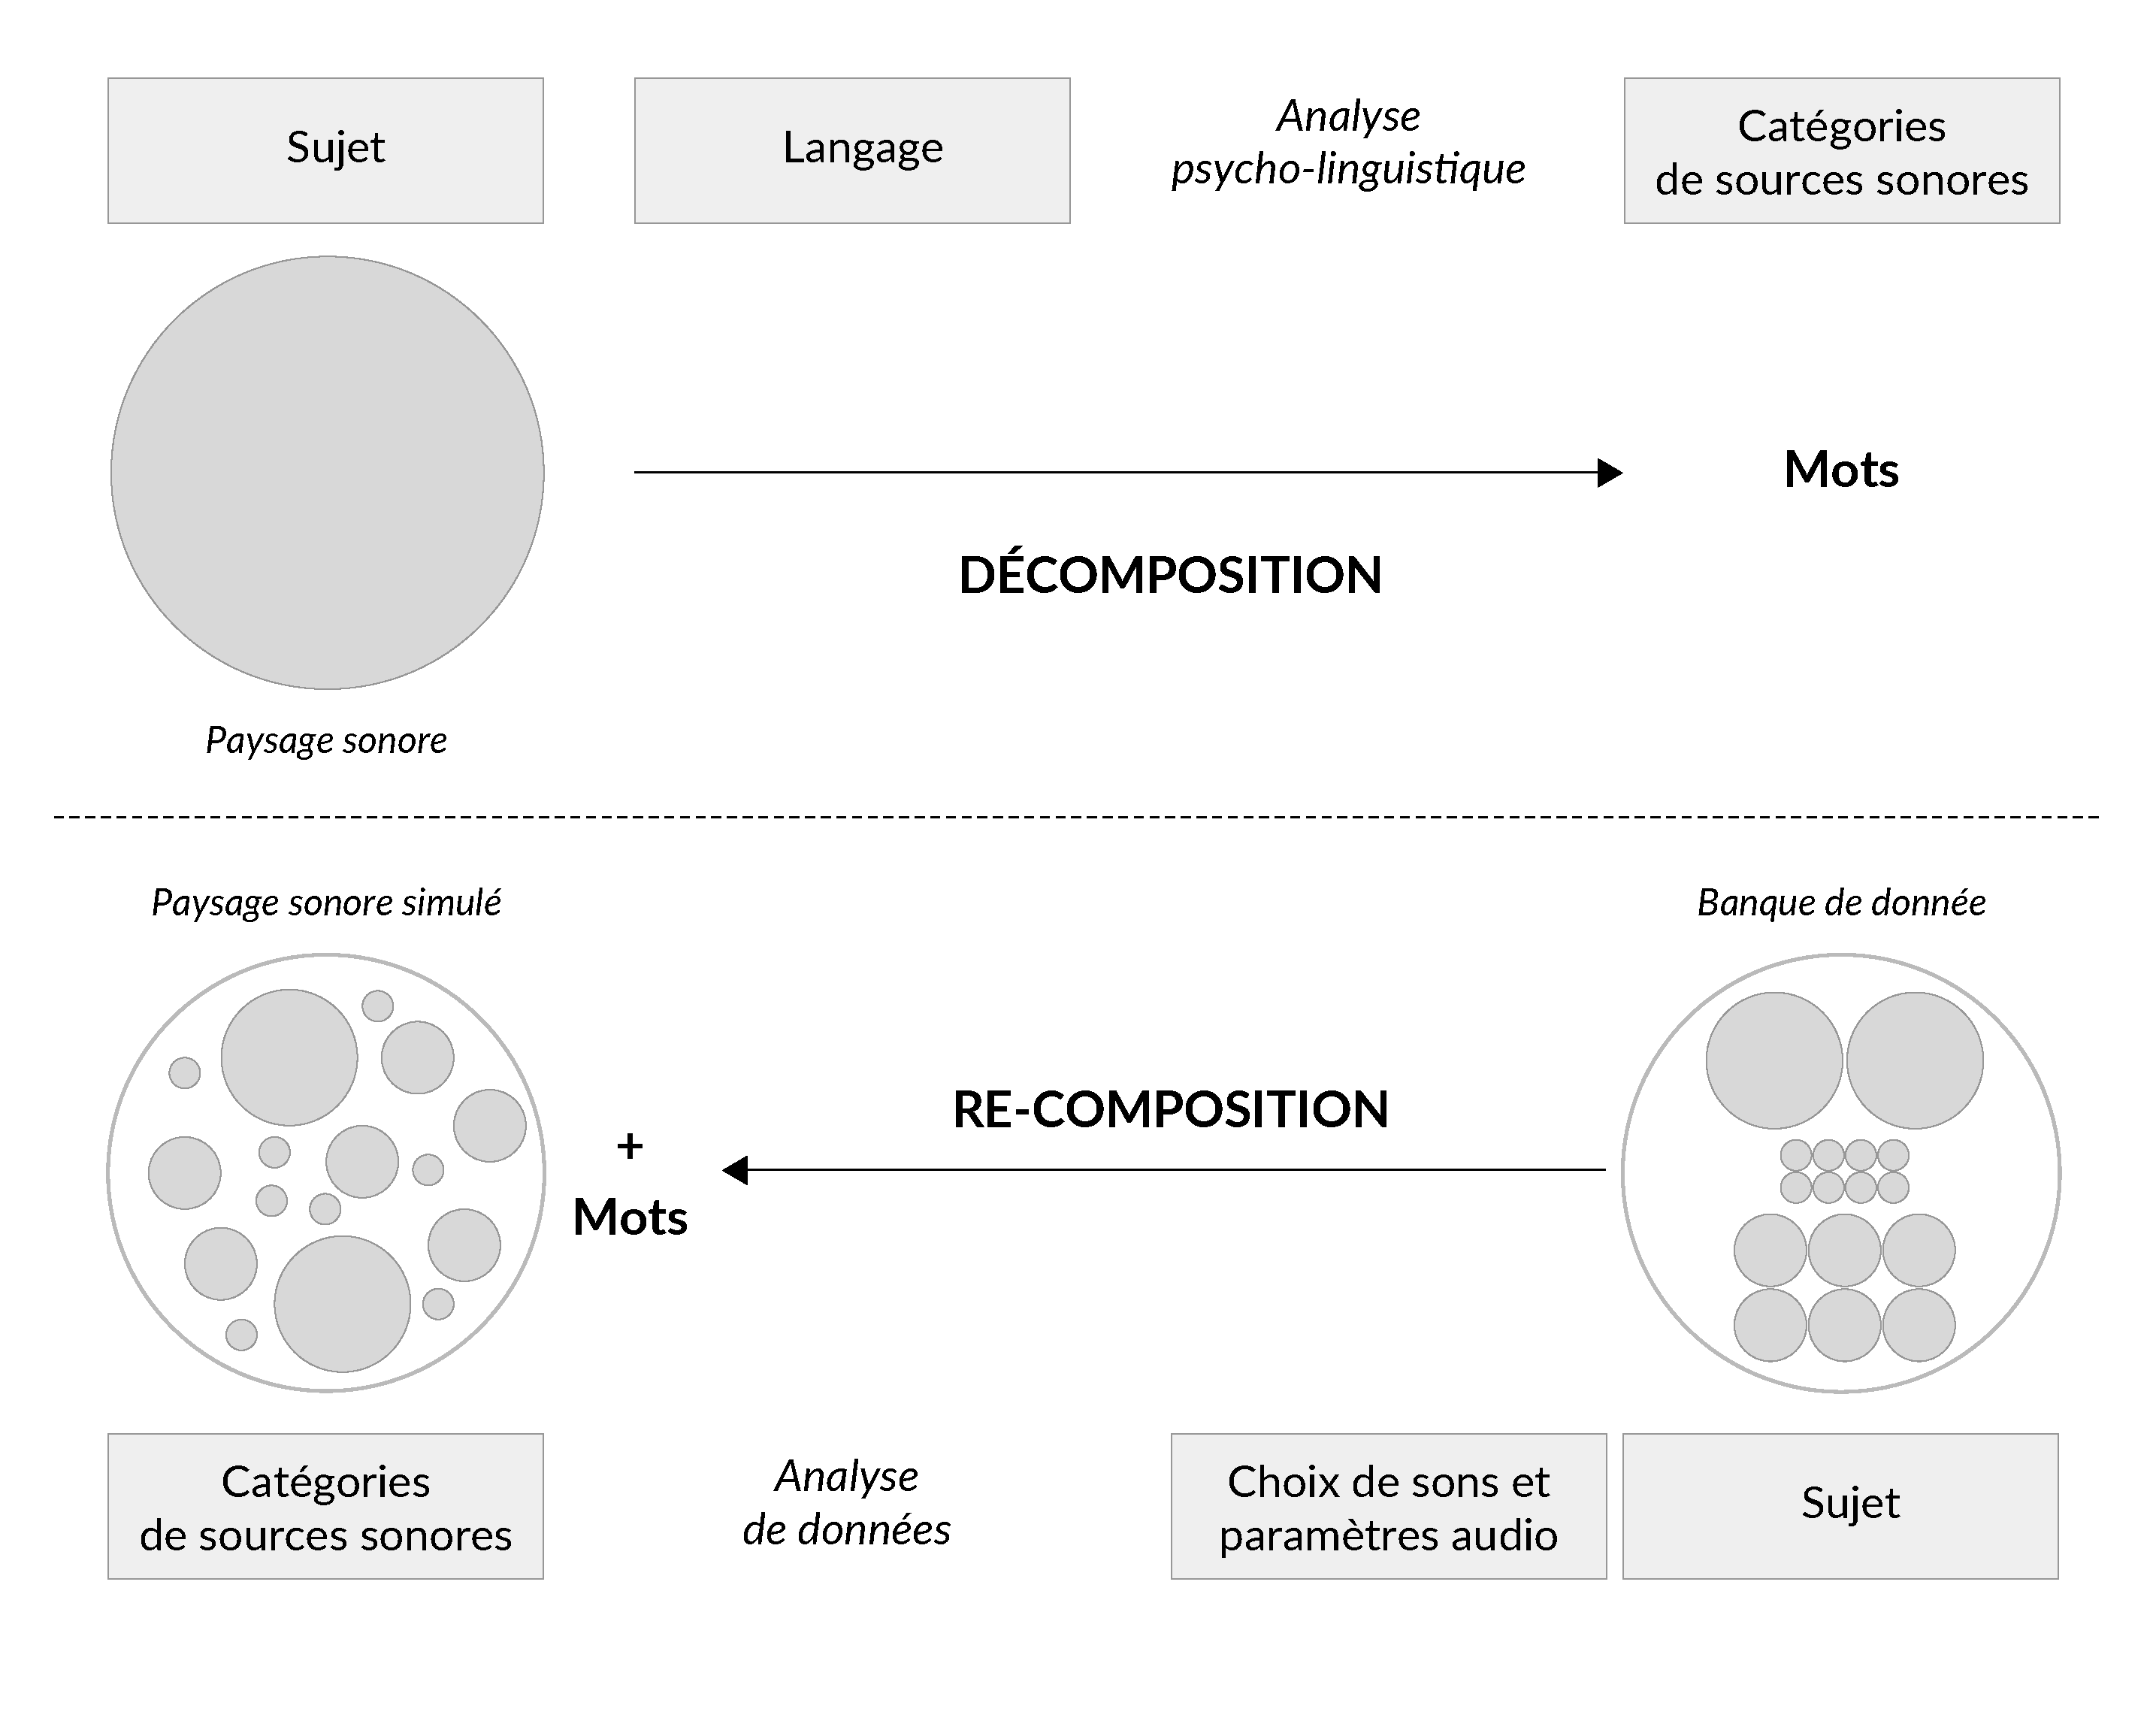
\includegraphics[width=.8\linewidth]{gfx/ch_4/1}
       \caption{Relation entre l'analyse psycholinguistique et la simulation.}\label{fig:paradigmeSimu1}
\end{figure}
 
\subsubsection{Utilisations antérieures de la simulation}

Plusieurs outils de simulation de scènes sonores ont déjà été proposés \citep{misra2006new,misra2007musical,valle2009framework,finney2010soundscape,schirosa2010system}. Ils ont souvent pour but de générer automatiquement l'ambiance sonore d'un environnement virtuel \citep{valle2009framework,finney2010soundscape}. Ils peuvent être vus comme des systèmes semi-autonomes: la simulation étant contrôlée par un utilisateur, mais dépendant aussi, soit d'un environnement visuel à illustrer, soit d'un environnement sonore à reproduire. D'autres outils, entièrement contrôlés par un utilisateur, servent, eux, d'aide à la composition \citep{misra2006new,misra2007musical}. Ces systèmes s'éloignent tous sensiblement du cadre expérimental de l'analyse sensorielle.

Bruce~\al \citep{bruce2009development,bruce2014effects} se sont servis de la simulation afin d'étudier la perception des paysages sonores. Ils proposent un système de simulation permettant au sujet d'agir sur un environnement en ajoutant ou supprimant des sources sonores spécifiques. Ce système permet par ailleurs de modifier le niveau sonore des sources, et leurs positions spatiales.

A l'aide de cet outil, les auteurs demandent à leurs sujets de manipuler des sources, afin de recréer un environnement urbain. Ce que faisant, ils montrent que l'inclusion ou l'exclusion des sources dépendent plus de considérations sociales/sémantiques, que des caractéristiques physiques des sources. Ils soulignent néanmoins que le manque d'enregistrements disponibles limite l'analyse. Ils suggèrent de regrouper les enregistrements similaires en «~groupes sémantiques~» afin de faciliter l'analyse, ce qui est fait dans le cas de notre modèle. 

En utilisant le simulateur proposé par \citep{bruce2009development}, \citep{davies2014soundscape} montrent que, lorsqu'on demande à des participants de simuler un environnement sonore, les simulations font référence à ce que ces derniers s'imaginent être un environnement typique, sans tenir compte de leurs propres préférences pour des sources sonores particulières. Les auteurs soulignent là encore que le faible nombre de sources disponibles (16), ainsi que le nombre réduit de paramètres de contrôle (niveaux des sources, positions spatiales), limitent l'expressivité du sujet, et par conséquent, les capacités de l'analyse.

Dans notre démarche, nous faisons le choix d'une restitution simplifiée (monophonique) des scènes, au profit d'un nombre plus important de paramètres et de sources disponibles, ce afin de garantir, à la sortie, des données viables et expressives.

\subsection{Simulation et détection automatique d'événements sonores}
\label{sec:ch4_modAnaAuto}

En apprentissage machine, la valeur des systèmes proposés par la communauté est bien souvent indexée sur les performances obtenues par ces systèmes sur des corpus d'évaluation.

Comme nous l'avons évoqué à la section~\ref{ch1_SED}, un corpus mal construit, \ie~présentant une caractéristique cachée, sur/sous représentée, peut entraîner des erreurs d'interprétations importantes. Pour limiter ces biais potentiels, deux approches peuvent être envisagées:

\begin{itemize}
\item augmenter le nombre des données, afin que les biais potentiels se retrouvent «~dilués~» face à la diversité des données proposées;
\item considérer des données très contrôlées.
\end{itemize}

La première approche est celle suivie habituellement dans l'évaluation des algorithmes d'analyse automatique. La deuxième, consistant à travailler avec des données peu nombreuses, mais maîtrisées, tient plutôt des pratiques expérimentales ayant cours en analyse sensorielle, ou, par définition, il n'est pas envisageable de soumettre le sujet à un trop grand nombre de stimuli.

C'est cette deuxième approche que nous suivons afin d'évaluer les algorithmes de détection automatique d'événements sonores. Nous nous appuyons sur le modèle proposé pour générer des scènes dont nous maîtrisons les caractéristiques structurelles, à savoir:

\begin{itemize}
\item le nombre de classes;
\item le nombre d'événements par classe;
\item le rapport entre le niveau sonore de l'événement et celui du \emph{background}. 
\end{itemize}

Le nombre et la nature des classes sont déterminés par la typologie de la banque de données. Dans le cadre de l'analyse automatique, la typologie n'a cependant pas besoin d'être organisée en une structure taxonomique, le nombre de classes d'événements étant souvent assez faible.

Le nombre d'événements par classe est une résultante directe de l'espacement inter-\emph{onset}. Comme nous le verrons par la suite, nous considérons également une variante du modèle où le nombre d'événements est directement contrôlé (\cf~Section~\ref{sec:ch7_simulationDcase2016}).

Enfin, une propriété essentielle de tout algorithme de détection est d'être robuste à différents niveaux de bruit de fond (\emph{background}). Le bruit ici est représenté par l'ensemble des sons n'appartenant pas aux classes à détecter. Dans le modèle présenté, les classes d'événements sont modélisées par des pistes d'événements, tandis que le bruit de fond est modélisé par une unique piste de \emph{texture}. Dans le cas de l'analyse sensorielle, les facteurs $\mu^a_i$ et $\sigma^a_i$ déterminant l'amplitude des samples d'événements de la classe $i$ ne déterminent pas le niveau sonore absolu d'un sample, mais le rapport entre le niveau de ce sample, et celui du \emph{background}.

Nous invitons le lecteur à se référer aux sections~\ref{sec:ch7_simuProcessInstance}, \ref{sec:ch7_simuProcessAbstract} et~\ref{sec:ch7_simulationDcase2016} pour une description détaillée des différents processus de simulation utilisés pour générer les corpus de scènes dans le cadre de l'évaluation des algorithmes de détection automatique d'événements.

\section{Conclusion}

Dans ce chapitre, nous introduisons un modèle fondé sur des considérations perceptives. Le modèle est pensé afin de faciliter la génération de données simulées. Concernant l'analyse sensorielle, nous montrons en quoi la simulation permet de capturer la représentation mentale que se fait un individu d'un environnement en particulier, et motivons son utilisation dans le cadre des études sur les paysages sonores urbains. Concernant l'analyse automatique, nous montrons l'importance de considérer des scènes dont la structure des séquences d'événements est contrôlée par l'expérimentateur, afin de finement apprécier les performances des algorithmes de détection d'événements sonores.

Les deux chapitres suivant présentent les deux cas d'étude.
%*****************************************
%*****************************************
%*****************************************
%*****************************************
%*****************************************

